\documentclass[]{article}
\usepackage[utf8]{inputenc}
\usepackage[english,russian]{babel}
%\usepackage[12pt]{extsizes}
\usepackage{amsmath}
\usepackage{enumerate}

%\usepackage[left=3cm, top=1.5cm, right=1.3cm, bottom=2cm, nohead, footskip=10mm]{geometry}
\usepackage[12pt]{extsizes}
\linespread{1.3}
\usepackage[left=3cm, top=1.5cm, right=1.3cm, bottom=2cm, nohead, footskip=10mm]{geometry}


\usepackage[absolute,overlay]{textpos}
\usepackage{indentfirst}
\usepackage{float}
\restylefloat{table}
\usepackage{hyperref}
\usepackage{mathtext}
\usepackage{amsfonts}
\usepackage{amsthm}
\usepackage{tikz}
\usepackage{xspace}
\usetikzlibrary{shapes,positioning,shadows,trees,automata,arrows.meta,shapes.geometric}
\usepackage{pgf-pie}
\usepackage{chngcntr}
\usepackage{pdfpages}
\usepackage{systeme}
\usepackage{empheq}
\numberwithin{equation}{section}
\usepackage{caption}
\DeclareCaptionLabelSeparator{none}{. }
\captionsetup{labelsep=none}


\pagestyle{plain}

\begin{document}
    \thispagestyle{empty}
	\begin{center}
		Министерство образования и науки Российской Федерации\\
		Санкт-Петербургский государственный технический университет\\
		Институт прикладной математики и механики\\
		Кафедра <<Телематика>>\\
		\vspace{5cm}
		\textbf{\textbf{ЛАБОРАТОРНАЯ РАБОТА}}\\
        \vspace{0.5cm}
        \textbf{ПО ТЕМЕ}\\
        \vspace{0.5cm}
		\textbf{\textbf{<<Наивный Байесовский классификатор>>}}\\
		\vspace{3cm}
		по направлению 02.04.01.02 <<Организация и управление суперкомпьютерными системами>>
	\end{center}
	\vspace{2cm}
	\begin{tabular} {l l l}
	\hspace{9.5cm} & Выполнил: & \\
	& Студент гр. 13643.1 & Титов А.И.\\
	& Проверил: & Уткин Л.В.
	\end{tabular}
	\vspace{4.5cm}
	\begin{center}
		Санкт-Петербург\\
		2019
    \end{center}


	\renewcommand\contentsname{Оглавление}
	\tableofcontents

    \newpage
    \section*{Постановка задачи}
    \addcontentsline{toc}{section}{Постановка задачи}

    Требуется выполнить следующие задачи:
    \begin{enumerate}
        \item Исследовать, как объем обучающей выборки и количество тестовых данных, влияет на точность классификации или на вероятность ошибочной классификации в примере крестики-нолики и примере о спаме e-mail сообщений.
        \item Сгенерировать 100 точек с двумя признаками X1 и X2 в соответствии с нормальным распределением так, что первые 50 точек (class -1) имеют параметры: мат. ожидание X1  равно 10, мат. ожидание X2 равно 14, среднеквадратические отклонения для обеих переменных равны 4. Вторые 50 точек (class +1) имеют параметры: мат. ожидание X1 равно 20, мат. ожидание X2 равно 18, среднеквадратические отклонения для обеих переменных равны 3. Построить соответствующие диаграммы, иллюстрирующие данные. Построить байесовский классификатор и оценить качество классификации.
        \item Разработать байесовский классификатор для данных Титаник (Titanic dataset).
    \end{enumerate}

    \newpage
    \section{Крестики-нолики и спам e-mail сообщений}
        Для того чтобы исследовать, как объем обучающей выборки влияет на точность классификации были проделаны следующие шаги:

        \begin{enumerate}
            \item Загрузка и препроцессинг исходных данных из файла в структуру \textbf{data\_frame}. Для хранения и препроцессинга использован пакет \textit{pandas}.
            \item Инициализация классификатора \textit{GaussianNB} из пакета \textit{sklearn}.
            \item Выполнение цикла по разбиению соотношения обучающей и тестовой выборки от 0.1 до 0.9 с количеством шагов - 10. Разбиение производится с помощью метода \textit{train\_test\_split} из пакета \textit{sklearn}.
            \item Применение классификатора к каждому разбиению. На данном этапе происходит основная часть вычислений:
                \begin{itemize}
                    \item рандомизация исходных данных;
                    \item использование наивного Байесовского классификатора для вычисления условных апостериорных вероятностей категориальных переменных при условии независимости признаков;
                    \item оценка полученной модели;
                    \item сравнение прогнозируемых значений с исходными;
                    \item вычисление значения вероятности ошибочной классификации.
                \end{itemize}
            \item Далее происходит построение графика зависимости значения вероятности ошибочной классификации от объема обучающей выборки.
            \item Также выводится таблица, отображающая ошибки кластеризации для разбиения исходной выборки с соотношением обучающей выборки к тестовой 0.8.
        \end{enumerate}

        Вычисления производились на двух выборках: крестики-нолики и спам e-mail сообщений. Соответственно, в результате получилось 2 графика (см. Рис.1-2). А также получена таблица, отображающая ошибки кластеризации для разбиения исходной выборки с соотношением обучающей выборки к тестовой 0.8. (см. таблица 1-2)

        \begin{figure}[H]
            \centering
            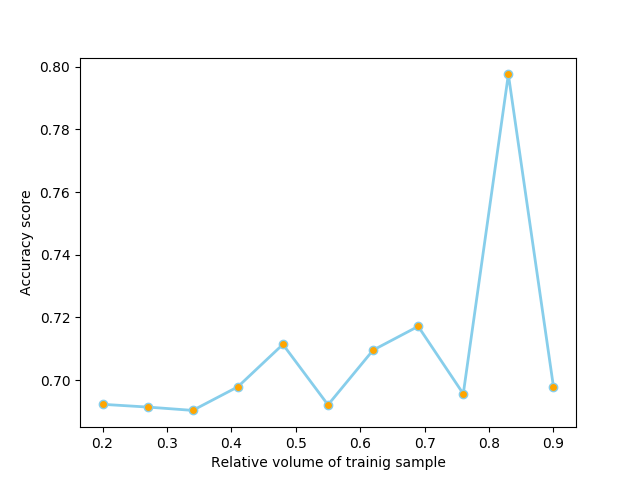
\includegraphics[width = 0.8\linewidth]{data/tic_tac_toe.png}
            \caption{График зависимости для примера <<Крестики-нолики>>}
        \end{figure}

        \begin{figure}[H]
            \centering
            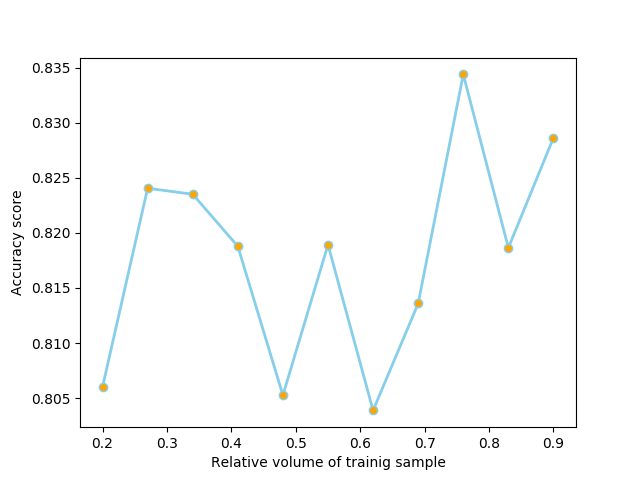
\includegraphics[width = 0.8\linewidth]{data/spam.png}
            \caption{График зависимости для примера <<Спам e-mail сообщений>>}
        \end{figure}

        \begin{table}[H]
            \centering
            \begin{tabular}{|c|c|c|}
              \hline
                & \textbf{0} & \textbf{1} \\
              \hline
              \textbf{0} & 129 & 0\\
              \hline
              \textbf{1} & 50 &  13\\
              \hline
            \end{tabular}
            \caption{Сравнение результатов с исходными данными (<<Крестики-нолики>>)}
        \end{table}

        \begin{table}[H]
            \centering
            \begin{tabular}{|c|c|c|}
              \hline
                & \textbf{0} & \textbf{1} \\
              \hline
              \textbf{0} & 382 & 166\\
              \hline
              \textbf{1} & 16 & 357 \\
              \hline
            \end{tabular}
            \caption{Сравнение результатов с исходными данными (<<Спам e-mail сообщений>>)}
        \end{table}

    \section{Сгенерированный dataset}
        Для построения Байесовского классификатора и оценки качества классификации выполнены следующие шаги:

        \begin{enumerate}
            \item Генерация двух векторов по 100 элементов согласно заданным параметрам.
            \item Составление таблицы из полученных векторов, а также назначение меток класса получившимся элементам.
            \item Рандомизация таблицы.
            Разбиение исходной выборки на обучающее и тестирующее множество.
            \item Использование наивного Байесовского классификатора для вычисления условных апостериорных вероятностей категориальных переменных при условии независимости признаков.
            \item Оценка полученной модели.
            \item Построение таблицы для сравнения прогнозируемых значений с исходными (см. таблица 3).
            \item Построение графика принадлежности сгенерированных точек определённому классу. (см. рис. 3)
            \item Построение графика зависимости значения вероятности ошибочной классификации от объема обучающей выборки. (см. рис. 4) (Аналогично предыдущей задаче)
        \end{enumerate}

        \begin{table}[H]
            \centering
            \begin{tabular}{|c|c|c|}
              \hline
                & \textbf{-1} & \textbf{1} \\
              \hline
              \textbf{-1} & 7 & 1\\
              \hline
              \textbf{1} & 0 & 12 \\
              \hline
            \end{tabular}
            \caption{Сравнение результатов с исходными данными (Сгенерированный dataset))}
        \end{table}

        Тестирующая выборка 20\% от исходной, следовательно для классификации было использовано 20 элементов. Анализируя Таблицу 3, можно сделать вывод о том, что лишь 1 значение было классифицировано неверно. Таким образом, величина ошибки для данного примера составила 0.05.

        \begin{figure}[H]
            \centering
            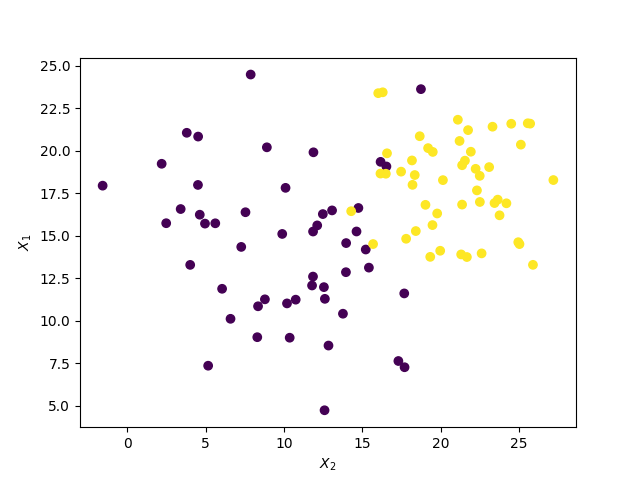
\includegraphics[width = 1.0\linewidth]{data/generated.png}
            \caption{График распределения данных для двух классов}
        \end{figure}

        \begin{figure}[H]
            \centering
            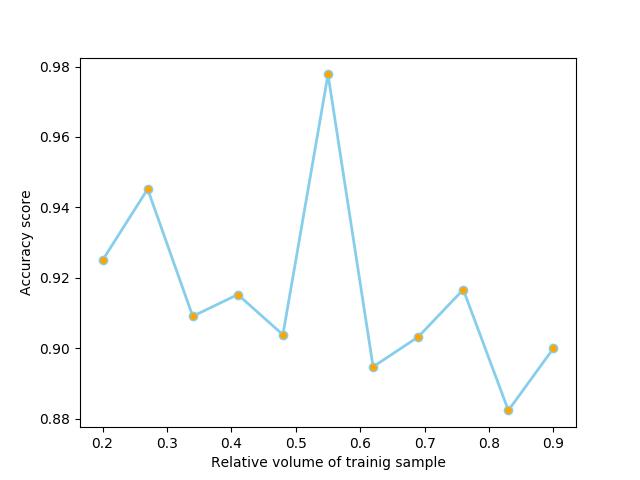
\includegraphics[width = 1.0\linewidth]{data/generated_precision.png}
            \caption{График зависимости для примера <<Сгенерированный dataset>>}
        \end{figure}

    \section{Titanic dataset}

    Для разработки байесовского классификатора для данных «Титаник» выполнены следующие шаги:

    \begin{enumerate}
        \item Загрузка и препроцессинг обучающей и тестирующей выборок в соответствующие таблицы.
        \item Использование наивного Байесовского классификатора для вычисления условных апостериорных вероятностей категориальных переменных при условии независимости признаков.
        \item Оценка полученной модели.
        \item Построение таблицы для сравнения прогнозируемых значений с исходными (см. таблица 4).
        \item Вычисление значения вероятности ошибочной классификации.
        \item Построение графика зависимости значения вероятности ошибочной классификации от объема обучающей выборки. (см. рис. 5) (Аналогично предыдущей задаче)
    \end{enumerate}

    \begin{table}[H]
        \centering
        \begin{tabular}{|c|c|c|}
          \hline
            & \textbf{0} & \textbf{1} \\
          \hline
          \textbf{0} & 221 & 45\\
          \hline
          \textbf{1} & 39 & 113 \\
          \hline
        \end{tabular}
        \caption{Сравнение результатов с исходными данными (Titanic dataset))}
    \end{table}

    Таким образом величина ошибочной классификации в примере составила $\approx0,21$. Стоит заметить, что на изначальная выборка тестовых данных была получена основываясь на гендерном признаке выживания (указано в источнике выборки \href{https://www.kaggle.com/c/titanic/}{https://www.kaggle.com/c/titanic/}).
    В данном примере обучение производилось по всем возможным колонкам, за исключением колонки <<Ticket>>, а также колонки <<SibSp>> и <<Parch>> были заменены на их сумму + 1 (колонка <<FamilySize>>), колонка <<Cabin>> была заменена на колонку с бинарными значениями <<HasCabin>>.

    \begin{figure}[H]
        \centering
        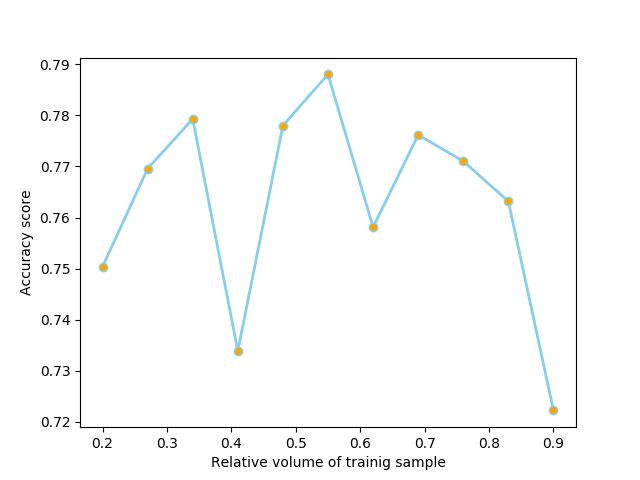
\includegraphics[width = 0.9\linewidth]{data/titanic.png}
        \caption{График зависимости для примера <<Titanic dataset>>}
    \end{figure}

\end{document}
